%!TEX root = ../hycas2010.tex
% Points in the input file are y-scaled by 0.5 so yval 1000 represents point 2000 in the original results. The reason for scaling was that TeX cannot handle > ~16k numbers
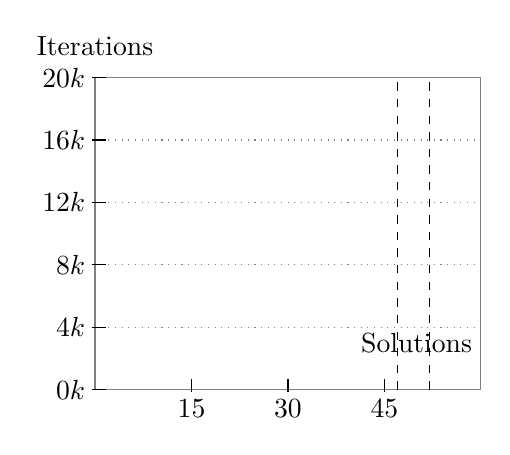
\begin{tikzpicture}[x=0.08166cm,y=0.0004cm]
    % Draw the axes and grid lines
    \draw[-,gray] (0,0) -- (0,10000) -- (60,10000) -- (60,0) -- cycle; 
    \draw[-,gray,thin, dotted, ystep=2000, xstep=60] (0,0) grid (60,10000);
    \foreach \x in {15, 30, 45}  \draw [-,xshift=0](\x,4pt) -- (\x,-1pt);
    \foreach \y in {0,2000,4000,6000,8000,10000}  \draw [-,yshift=0](4pt,\y) -- (-1pt,\y);
    \foreach \x/\xtext in {15/15, 30/30, 45/45} \node at (\x,0) [below] {$\xtext$};
    \foreach \y/\ytext in {0/0k,2000/4k,4000/8k,6000/12k,8000/16k,10000/20k}  \node at (0,\y) [left] {$\ytext$};
    \node at (0,11000) {Iterations};
    \node at (50,1500) {Solutions};
    \draw[-,gray] plot[mark=o,mark size=3,mark options={color=black}] 
			file {data/hanoi5s.CP.tikzdata};
    \draw[-,gray] plot[mark=x,mark size=4,mark options={color=black}] 
			file {data/hanoi5s.CF.tikzdata};
	\draw [-,dashed](47,0pt) -- (47,10000);
	\draw [-,dashed](52,0pt) -- (52,10000);
\end{tikzpicture}
